% !TeX spellcheck = en_US
\subsection{Direct encoding}
As the name suggests, the direct encoding assign for each CSP variable $x$ and for each possible value from its domain $i$ a new propositional variable $x_i$ on the SAT side. The boolean variable is then True if and only if the original variable is assigned the value $i$.  To ensure consistent logical assignment for each propositional variable, we need to extend the SAT problem to include clauses that avoid inconsistent results such as assigning a CSP variable two values at the same time or no value at all (at-least-once and at-most-once clauses) \cite{petke2011order}.

\subsubsection{Example}
Consider the following instance of the map coloring problem:\\
\begin{figure}[H]
	\centering
	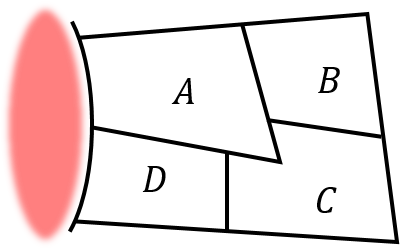
\includegraphics[width=0.5\linewidth]{assets/map_coloring_unsolved}
	\captionsetup{justification=centering,margin=2cm}
	\caption{Unsolved instance of the map coloring problem}
	\label{fig:map_coloring_unsolved}
\end{figure}  
The map consists of four regions $A,B,C,D$ sharing boarder as shown in the figure \ref{fig:map_coloring_unsolved}. The purpose of this problem is to color each region of the map so that no two adjacent regions have the same color. The variables in this case are the regions themselves $\{A,B,C,D\}$ and each of them has the domain $\{r,g,b\}$ which stands for the colors red, green and blue respectively. To fully define the CSP we also need to define the constraints' set which comprise two types of constraints: 
\begin{itemize}
	\item unary constraints such as $A\neq r$ since $A$ is already adjacent to a red colored region 
	\item binary constraints such as $A\neq B, A\neq C,\dots$ i.e. no two adjacent regions share the same color
\end{itemize}
Hereafter, the unary constraints are avoided by restricting the domain of $A$ and $D$ to not include red; on the other hand, it should be noted that usually all the variables are given the same domain to simplify the problem.

Encoding this problem directly will result in the following SAT instance:
a new propositional variable is associated with each value that can be assigned to a CSP variable. So we get the variables: $\{ A_g, A_b, B_r, B_g,\\ B_b, \dots\}$. To ensure that each CSP variable will be assigned at least one color, we have to include the following at-least-once (ALO) clauses: $\{ A_g \vee A_b, B_g \vee B_r \vee B_b, \dots \}$. Similarly, we must ensure that no CSP variable is assigned multiple colors at the same time, which can be expressed as these at-most-once (AMO) clauses: $\{ A_g \oplus A_b, B_g \oplus B_r, B_g \oplus B_b, B_r \oplus B_b, \dots \} $, where $\oplus$ stands for the logical exclusive or operation $a \oplus b \equiv (a \wedge \neg b) \vee (\neg a \wedge b) \equiv (a \vee b) \wedge \neg (a \wedge b)$.
\begin{figure}[H]
	\centering
	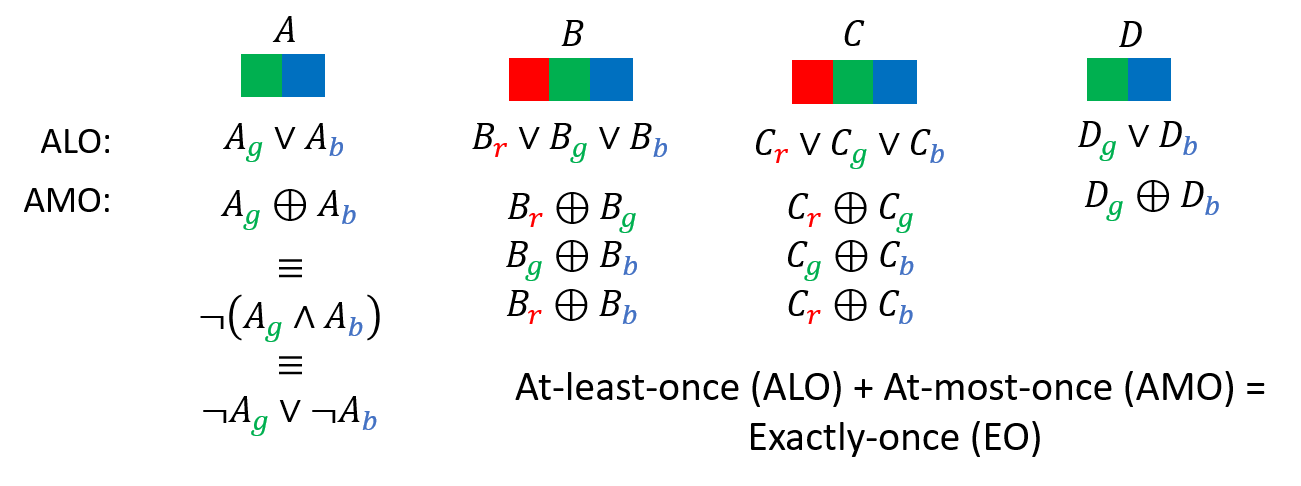
\includegraphics[width=0.75\linewidth]{assets/alo_amo}
	\captionsetup{justification=centering,margin=2cm}
	\caption{Both types of clauses in direct encoded SAT}
	\label{fig:alo_amo}
\end{figure}  
ALO and AMO clauses will enforce each CSP variable to be true only for one value from its domain, hence the name exactly-once (EO) clauses.

We still need to encode the binary constraints from CSP into some sort of clauses in SAT. This can be done easily by ensuring that no two CSP variables such as $C$ and $B$ share the same color, which can be translated into the following clauses:
$$
	\neg (C_r \wedge B_r) \quad, \neg (C_g \wedge B_g) \quad, \neg (C_b \wedge B_b)
$$
The same principle applies for the reset.
%\textcolor{red}{TODO: add a word about the similar support encoding (since both are sparse encodings)}

The direct encoding can be categorized under a general type called the sparse encoding. Notice that the direct encoding encodes conflict points (so called conflict or no-good) assignments such as $A$ and $B$ can't share the same color at the same time $\neg (A_c \wedge B_c) \equiv \neg A_c \vee \neg B_c$. It is also possible to encode the allowed (so called supports) assignments, e.g. $\neg A_c \vee B_c \vee C_c \vee D_c$. This type of clauses is the basis for the other type of sparse encoding called accordingly the support encoding \cite{petke2011order}.

\subsubsection{Proposition}
Solving the CSP problem directly with FC compared to the direct encoded SAT instance of the same CSP problem solved with DPLL will always result in similar search tree structure. i.e. FC on the original CSP problem and DPLL on the direct encoded SAT will explore the same number of branches. This proposition assumes equivalent branching heuristics for DPLL and FC.

\subsubsection{Proof idea}
Considering the generated search tree, our version of DPLL comprise only two rules: the one literal and the branching rule. This means at each node in the tree we either have to branch or the given variable must be assigned a truth value of either False or True. 

On the FC side branching is equivalent to its counterpart in DPLL. The second case in DPLL (unit propagation by the one literal rule) is also equivalent to applying forward checking by enforcing arc consistency and reducing the domain of each CSP variable to one value only.

Similarly, we can trace the whole structure of both trees and process with the same logic on each propositional variable. By induction, we can prove that each algorithm explore the same number of branches \cite{walsh2000sat}. 

\subsubsection{Example}
Compare the following search trees of FC applied to the previous map coloring problem and DPLL applied to direct encoded instance of the same previous map-coloring problem:
\begin{figure}[H]
	\centering
	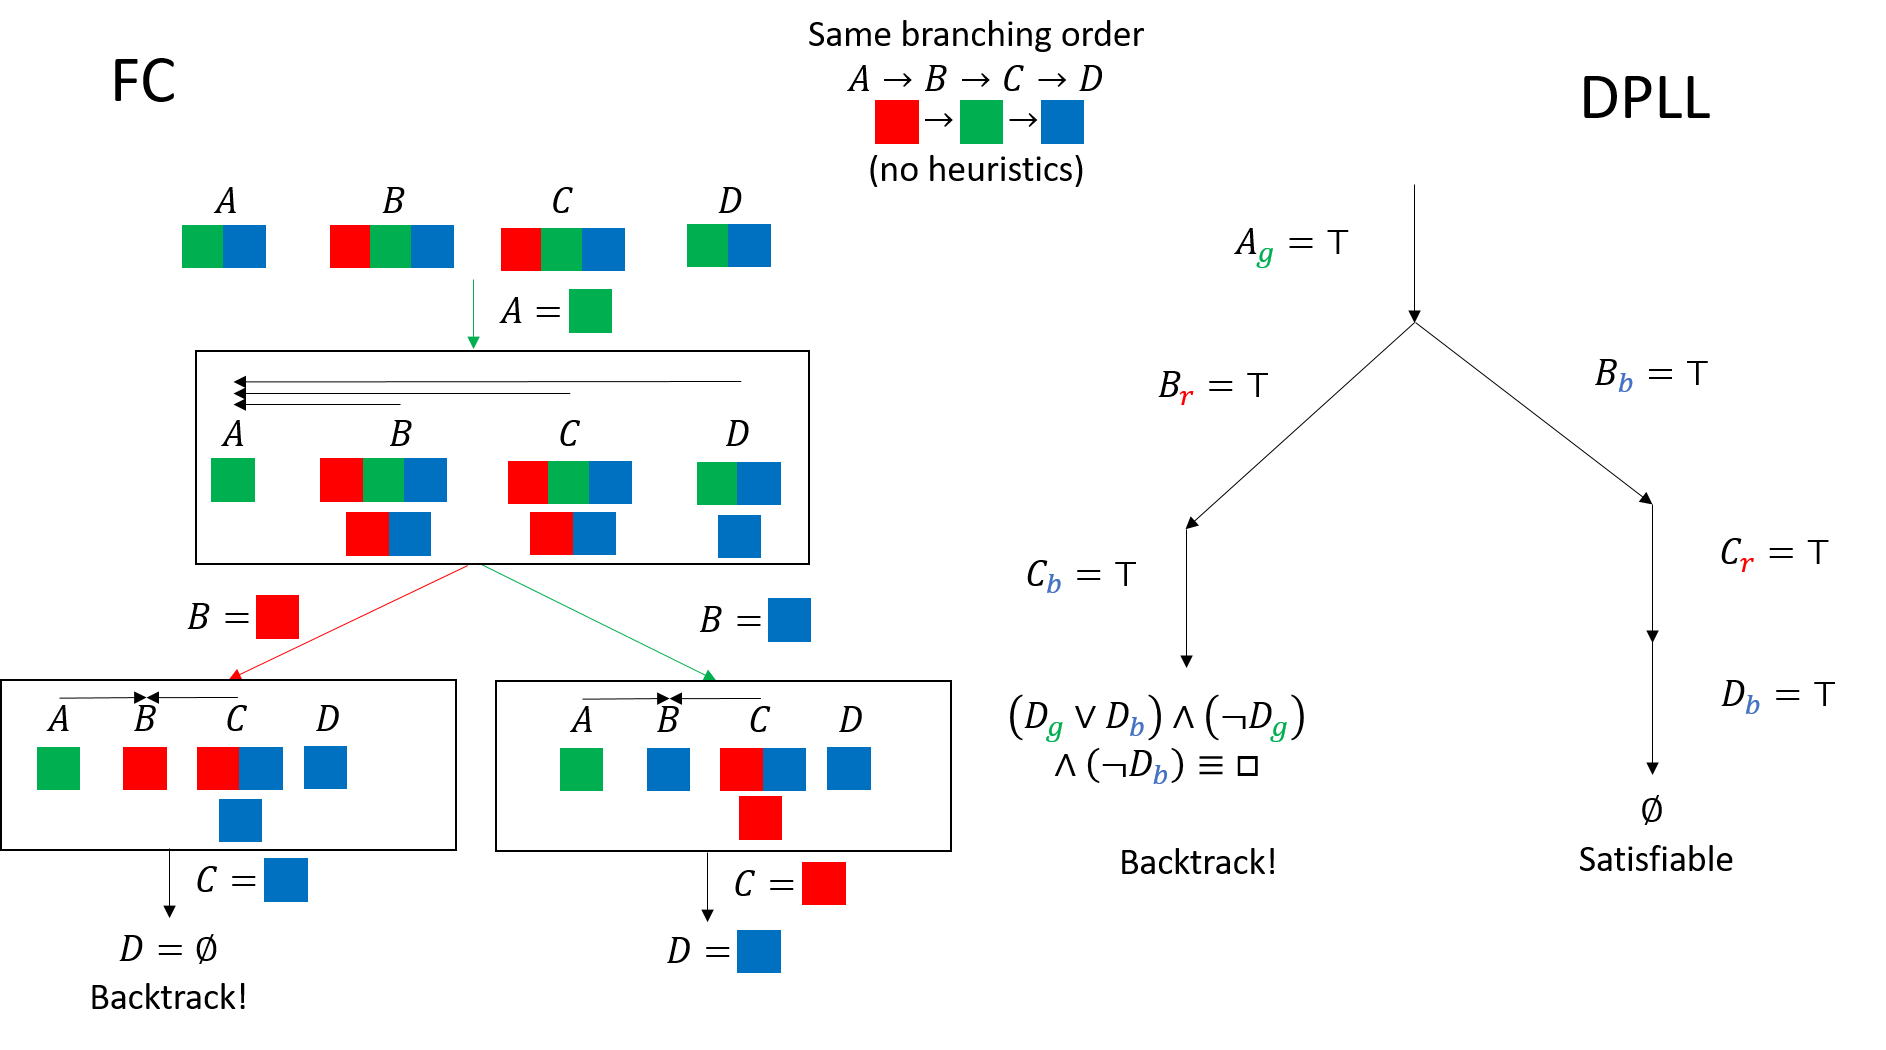
\includegraphics[width=1\linewidth]{assets/direct_fc_vs_dpll}
	\captionsetup{justification=centering,margin=2cm}
	\caption{Search trees of FC and DPLL}
	\label{fig:direct_fc_vs_dpll}
\end{figure} 
The arrows in node level on the FC side indicates enforcing arc consistency and the results are show directly underneath on the next line.



